\subsection{Unterraum der Differenzgesichter}
Seien nun $M,N\in\mathbb N$ fix.
Wir haben im letzten Kapitel gesehen, wie man schwarz-weiss Bilder der Auflösung $M\times N$ als Vektoren in $\mathbb R^{M\cdot N}$ verstehen kann.
Die Bilder müssen dafür nicht unbedingt ein Gesicht zeigen.
Die Pixel können sogar völlig zufällige Graustufen aufweisen, so dass auf dem Bild nichts sinnvolles zu erkennen ist.
Dies führt uns zu folgender Beobachtung:
Nur die wenigsten Vektoren in $\mathbb R^{M\cdot N}$ entsprechen einem Gesicht.
Wir wollen uns näher mit dieser Beobachtung befassen.

Sei $K\in\mathbb N$ die Anzahl aller Bilder von allen Personen unserer Datenbank.
Jedes Bild soll dabei die Auflösung $M\times N$ haben.
Wir betrachten alle Bilder der Datenbank als Vektoren $\vec b_1,\ldots,\vec b_K\in\mathbb R^{M\cdot N}$.
Diese Darstellung erlaubt uns, das \textit{Durchschnittsgesicht}, wir nennen es $\vec m\in\mathbb R^{M\cdot N}$, zu definieren
\begin{equation*}
	\vec m=\frac{1}{K}\left(\vec b_1+\ldots+\vec b_K\right).
\end{equation*}
Das Durchschnittsgesicht lässt sich wieder als Bild ausgeben.
Aber wie sieht so ein Durchschnittsgesicht aus?
Das werden wir in folgender Übung herausfinden.
\begin{aufgabe}
	Ergänzen Sie im File \texttt{eigenfaces.py} die Funktion \texttt{meanface(b\_list)}.
	Dabei ist \texttt{b\_list} die Liste der Länge $K$ der Vektoren $\vec b_1,\ldots,\vec b_K$.
	Der Rückgabewert soll das Durchschnittsgesicht $\vec m$ sein.
	Sie können die ihre Lösung überprüfen indem Sie das Skript \texttt{meanface\_test.py} laufen lassen.
	\textit{Hinweis:} Die Python Funktionen \texttt{len(...) und sum(...)} können nützlich sein.
\end{aufgabe}
\begin{losung*}
	Hier ist eine mögliche Lösung und das davon mit \texttt{meanface\_test.py} generierte Durchschnittsgesicht.\\[0.5cm]
	\begin{minipage}{0.45\textwidth}
\begin{lstlisting}[style=python]
def meanface(b_list):
	K = len(b_list)
	return sum(b_list) / K
\end{lstlisting}
	\end{minipage}\hfill
	\begin{minipage}{0.3\textwidth}\vspace{-1cm}
		\centering\hfill Durchschnittsgesicht:
	\end{minipage}
	\begin{minipage}{0.2\textwidth}\vspace{-1cm}
		\centering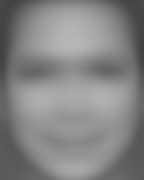
\includegraphics[width=0.6\textwidth]{images/facespace/meanface}
	\end{minipage}
\end{losung*}
Nachdem wir nun das Durchschnittsgesicht gebildet haben, berechnen wir nun die \textit{Differenzgesichter} $\vec a_1,\ldots,\vec a_K$.
Diese sind definiert als
\begin{equation*}
	\vec a_k=\vec b_k-\vec m,\quad k\in\left\{1,\ldots,K\right\}.
\end{equation*}
Die Methode der Eigengesichter trifft nun folgende Annahme:
Die Differenzgesichter sind in guter Approximation in einem niedrig-dimensionalen Unterraum von $\mathbb R^{M\cdot N}$ enthalten.
Wir nennen diesen Unterraum den \textit{Raum der Differenzgesichter} (engl. \textit{facespace}).
Sagen wir, dieser Unterraum habe die Dimension $D\ll M\cdot N$ (\glqq{}viel kleiner als\grqq{}).
Leider können wir das nur stark vereinfacht in für den Fall $M\cdot N=2$ und $D=1$ darstellen.
Dies ist in Abbildung~\ref{fig:meandiff} gezeigt.
\begin{figure}[ht]
	\centering
	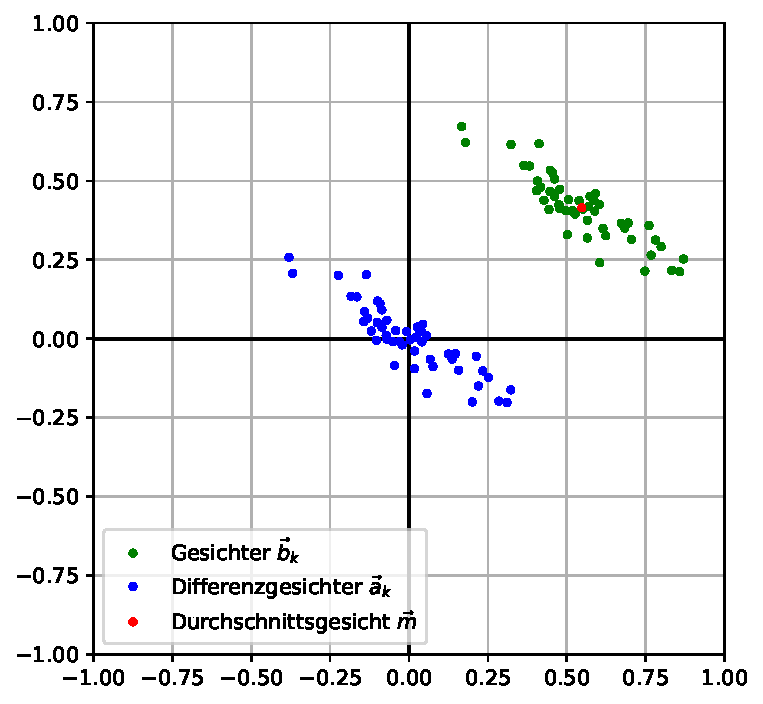
\includegraphics[width=0.5\textwidth]{images/facespace/meandiff}
	\caption{Die Gesichter werden um den Ursprung zentriert indem man das Durchschnittsgesicht subtrahiert.
	Annahme: Die entstehenden Differenzgesichter liegen dann in guter Approximation in einem Unterraum.}
	\label{fig:meandiff}
\end{figure}
\begin{aufgabe}
	Nennen Sie einen Unterschied und eine Gemeinsamkeit der vereinfachten Darstellung in Abbildung~\ref{fig:meandiff} zu unserer tatsächlichen Situation mit Bildern von Gesichtern.
	Gehen Sie davon aus, dass unsere Bilder eine Auflösung von $M=180$ und $N=144$ haben, wie im letzten Kapitel.
\end{aufgabe}
\begin{losung*}
	Als Vektoren aufgefasst sind die Gesichter Punkte im $\mathbb R^{M\cdot N}$.
	Für $M=180$ und $N=144$ wären das Punkte im $\mathbb R^{25'920}$ und nicht im $\mathbb R^2$ wie in der Abbildung.
	Der Unterraum der Differenzgesichter ist zudem dargestellt als Gerade durch Null, also als 1-dimensionaler Raum.
	Wegen der Vielfalt menschlicher Gesichter wird die Dimension tatsächlich viel grösser sein.
	Andererseits wird in der Abbildung korrekt gezeigt, dass das der Durchschnitt der Differenzgesichter der Nullvektor ist.
	Die Differenzgesichter sind also \glqq{}um Null verteilt\grqq{}.
\end{losung*}